%% (pdf)latex + bibtex + (pdf)latex + (pdf)latex [+ preview]
%%  F6 + F11 + F6 + F6 [+ F7]

%% abtex2-modelo-trabalho-academico.tex, v-1.9.6 laurocesar
%% Copyright 2012-2016 by abnTeX2 group at http://www.abntex.net.br/ 
%%
%% This work may be distributed and/or modified under the
%% conditions of the LaTeX Project Public License, either version 1.3
%% of this license or (at your option) any later version.
%% The latest version of this license is in
%%   http://www.latex-project.org/lppl.txt
%% and version 1.3 or later is part of all distributions of LaTeX
%% version 2005/12/01 or later.
%%
%% This work has the LPPL maintenance status `maintained'.
%% 
%% The Current Maintainer of this work is the abnTeX2 team, led
%% by Lauro César Araujo. Further information are available on 
%% http://www.abntex.net.br/
%%
%% This work consists of the files abntex2-modelo-trabalho-academico.tex,
%% abntex2-modelo-include-comandos and abntex2-modelo-references.bib
%%

% ------------------------------------------------------------------------
% ------------------------------------------------------------------------
% abnTeX2: Modelo de Trabalho Academico (tese de doutorado, dissertacao de
% mestrado e trabalhos monograficos em geral) em conformidade com 
% ABNT NBR 14724:2011: Informacao e documentacao - Trabalhos academicos -
% Apresentacao
% ------------------------------------------------------------------------
% ------------------------------------------------------------------------

\documentclass[
	% -- opções da classe memoir --
	12pt,				% tamanho da fonte
	openright,			% capítulos começam em pág ímpar (insere página vazia caso preciso)
    twoside,			% para impressão em recto e verso. Oposto a oneside
	a4paper,			% tamanho do papel. 
	% -- opções da classe abntex2 --
	%chapter=TITLE,		% títulos de capítulos convertidos em letras maiúsculas
	%section=TITLE,		% títulos de seções convertidos em letras maiúsculas
	%subsection=TITLE,	% títulos de subseções convertidos em letras maiúsculas
	%subsubsection=TITLE,% títulos de subsubseções convertidos em letras maiúsculas
	% -- opções do pacote babel --
	english,			% idioma adicional para hifenização
	french,				% idioma adicional para hifenização
	spanish,			% idioma adicional para hifenização
	brazil				% o último idioma é o principal do documento
	]{abntex2}


% ---
% Pacotes básicos 
% ---
\usepackage{lmodern}			% Usa a fonte Latin Modern			
\usepackage[T1]{fontenc}		% Selecao de codigos de fonte.
\usepackage[utf8]{inputenc}		% Codificacao do documento (conversão automática dos acentos)
\usepackage{lastpage}			% Usado pela Ficha catalográfica
\usepackage{indentfirst}		% Indenta o primeiro parágrafo de cada seção.
\usepackage{color}				% Controle das cores
\usepackage{graphicx}			% Inclusão de gráficos
\usepackage{microtype} 			% para melhorias de justificação
% ---
		
% ---
% Pacotes adicionais, usados apenas no âmbito do Modelo Canônico do abnteX2
% ---
\usepackage{lipsum}				% para geração de dummy text
% ---

% ---
% Pacotes para escrita matemática
% ---
\usepackage{amsmath}

\usepackage{amssymb}	 % qed
\usepackage{amsthm}      % Teoremas

\newtheorem{teorema}{Teorema}
\newtheorem{lema}{Lema}
\newtheorem{definicao}{Definição}

% Resetar o numberador de lemas no fim de todo capítulo
% Isso faz com que a numeração seja indexada por capítulos e não
% pelo documento todo
\numberwithin{lema}{chapter}
% Idem ao de cima, com teoremas/definições
\numberwithin{teorema}{chapter}
\numberwithin{definicao}{chapter}
% Idem aos anteriores com o ambiente figure
\numberwithin{figure}{chapter}

% PGF
\usepackage{pgf,tikz,pgfplots}
\pgfplotsset{compat=1.15}
\usepackage{mathrsfs}
\usetikzlibrary{arrows}
\usepackage{standalone}

% ---
% Pacotes de citações
% ---
\usepackage[brazilian,hyperpageref]{backref}	 % Paginas com as citações na bibl
\usepackage[alf]{abntex2cite}	% Citações padrão ABNT
% --- 
% CONFIGURAÇÕES DE PACOTES
% --- 

% ---
% Configurações do pacote backref
% Usado sem a opção hyperpageref de backref
\renewcommand{\backrefpagesname}{Citado na(s) página(s):~}
% Texto padrão antes do número das páginas
\renewcommand{\backref}{}
% Define os textos da citação
\renewcommand*{\backrefalt}[4]{
	\ifcase #1 %
		Nenhuma citação no texto.%
	\or
		Citado na página #2.%
	\else
		Citado #1 vezes nas páginas #2.%
	\fi}%
% ---

% ---
% Informações de dados para CAPA e FOLHA DE ROSTO
% ---
\titulo{\textbf{Cálculo Variacional}}
\autor{EDUARDO JOSÉ DE OLIVEIRA}
\local{Anápolis}
\data{2018}
\orientador{Prof. Me. Tiago de Lima Bento Pereira}
%\coorientador{Titulação e Nome do coorientador}
\instituicao{%
Universidade Estadual de Goiás
  \par
Câmpus Anápolis de Ciências Exatas e Tecnológicas Henrique Santillo
  \par
Curso de Matemática}
\tipotrabalho{Trabalho de Curso (Graduação)}
% O preambulo deve conter o tipo do trabalho, o objetivo, 
% o nome da instituição e a área de concentração 
\preambulo{Trabalho de Curso (TC) apresentado a Coordenação Adjunta de TC, como parte dos requisitos para obtenção do título de Graduado no Curso de Matemática da Universidade Estadual de Goiás.} %sob a orientação do Professor(a) titulação e nome do professor(a).}
% ---


% ---
% Configurações de aparência do PDF final

% alterando o aspecto da cor azul
\definecolor{blue}{RGB}{41,5,195}

% informações do PDF
\makeatletter
\hypersetup{
     	%pagebackref=true,
		pdftitle={\@title}, 
		pdfauthor={\@author},
    	pdfsubject={\imprimirpreambulo},
	    pdfcreator={LaTeX with abnTeX2},
		pdfkeywords={abnt}{latex}{abntex}{abntex2}{trabalho acadêmico}, 
		colorlinks=false,       		% false: boxed links; true: colored links
    	linkcolor=blue,          	% color of internal links
    	citecolor=blue,        		% color of links to bibliography
    	filecolor=magenta,      		% color of file links
		urlcolor=blue,
		bookmarksdepth=4
}
\makeatother
% --- 

% --- 
% Espaçamentos entre linhas e parágrafos 
% --- 

% O tamanho do parágrafo é dado por:
\setlength{\parindent}{1.3cm}

% Controle do espaçamento entre um parágrafo e outro:
\setlength{\parskip}{0.2cm}  % tente também \onelineskip

% ---
% compila o indice
% ---
\makeindex
% ---
\usepackage{CUSTOMIZACOES} %MEU 
\usepackage{helvet} %Meu importa uma fonte nova "sem serifa"
\usepackage{pdfpages}
% ----
% Início do documento
% ----
\begin{document}

% Seleciona o idioma do documento (conforme pacotes do babel)
%\selectlanguage{english}
\selectlanguage{brazil}

% Retira espaço extra obsoleto entre as frases.
\frenchspacing 

\iffalse
% ----------------------------------------------------------
% ELEMENTOS PRÉ-TEXTUAIS
% ----------------------------------------------------------
\pretextual

% ---
% Capa
% ---

\imprimircapa
% ---

% ---
% Folha de rosto
% (o * indica que haverá a ficha bibliográfica)
% ---
\imprimirfolhaderosto*
% ---

% ---
% Inserir a ficha bibliografica
% ---

% Isto é um exemplo de Ficha Catalográfica, ou ``Dados internacionais de
% catalogação-na-publicação''. Você pode utilizar este modelo como referência. 
% Porém, provavelmente a biblioteca da sua universidade lhe fornecerá um PDF
% com a ficha catalográfica definitiva após a defesa do trabalho. Quando estiver
% com o documento, salve-o como PDF no diretório do seu projeto e substitua todo
% o conteúdo de implementação deste arquivo pelo comando abaixo:
%
% \begin{fichacatalografica}
%     \includepdf[pages=1]{fig_ficha_catalografica.pdf}
% \end{fichacatalografica}

\begin{fichacatalografica}
	\sffamily
	\vspace*{\fill}					% Posição vertical
	\begin{center}					% Minipage Centralizado
	\fbox{\begin{minipage}[c][8cm]{13.5cm}		% Largura
	\small
	\imprimirautor
	%Sobrenome, Nome do autor
	
	\hspace{0.5cm} \imprimirtitulo  / \imprimirautor. --
	\imprimirlocal, \imprimirdata-
	
	\hspace{0.5cm} \pageref{LastPage} p. : il. (algumas color.) ; 30 cm.\\
	
	\hspace{0.5cm} \imprimirorientadorRotulo~\imprimirorientador\\
	
	\hspace{0.5cm}
	\parbox[t]{\textwidth}{\imprimirtipotrabalho~--~\imprimirinstituicao,
	\imprimirdata.}\\
	
	\hspace{0.5cm}
		1. Palavra-chave1.
		2. Palavra-chave2.
		2. Palavra-chave3.
		I. Orientador.
		II. Universidade xxx.
		III. Faculdade de xxx.
		IV. Título 			
	\end{minipage}}
	\end{center}
\end{fichacatalografica}
% ---

% ---
% Inserir errata
% ---
\begin{errata}
Elemento opcional da \citeonline[4.2.1.2]{NBR14724:2011}. Exemplo:

\vspace{\onelineskip}

FERRIGNO, C. R. A. \textbf{Tratamento de neoplasias ósseas apendiculares com
reimplantação de enxerto ósseo autólogo autoclavado associado ao plasma
rico em plaquetas}: estudo crítico na cirurgia de preservação de membro em
cães. 2011. 128 f. Tese (Livre-Docência) - Faculdade de Medicina Veterinária e
Zootecnia, Universidade de São Paulo, São Paulo, 2011.

\begin{table}[htb]
\center
\footnotesize
\begin{tabular}{|p{1.4cm}|p{1cm}|p{3cm}|p{3cm}|}
  \hline
   \textbf{Folha} & \textbf{Linha}  & \textbf{Onde se lê}  & \textbf{Leia-se}  \\
    \hline
    1 & 10 & auto-conclavo & autoconclavo\\
   \hline
\end{tabular}
\end{table}

\end{errata}
% ---

% ---
% Inserir folha de aprovação
% ---

% Isto é um exemplo de Folha de aprovação, elemento obrigatório da NBR
% 14724/2011 (seção 4.2.1.3). Você pode utilizar este modelo até a aprovação
% do trabalho. Após isso, substitua todo o conteúdo deste arquivo por uma
% imagem da página assinada pela banca com o comando abaixo:
%
% \includepdf{folhadeaprovacao_final.pdf}
%
\begin{folhadeaprovacao}

  \begin{center}
  {\ABNTEXchapterfont\bfseries\large\imprimirtitulo}
%    {\ABNTEXchapterfont\large\imprimirautor}

    \vspace*{\fill}\vspace*{\fill}
    \begin{center}
    {\ABNTEXchapterfont\large\imprimirautor}
%      \ABNTEXchapterfont\bfseries\Large\imprimirtitulo
    \end{center}
    \vspace*{\fill}
    
%    \hspace{.45\textwidth}
%    \begin{minipage}{.5\textwidth}
%        \imprimirpreambulo
%    \end{minipage}%
%    \vspace*{\fill}
\end{center}
\vfill  
      
   Trabalho de Curso de Matemática apresentado à Banca Examinadora como parte dos requisitos para a obtenção do grau de graduado em Licenciatura em Matemática. 
   
   Banca Examinadora do Trabalho de Curso de Matemática do Câmpus Anápolis de Ciências Exatas e Tecnológicas Henrique Santillo da Universidade Estadual de Goiás, \imprimirlocal, 10 de agosto de 2018.

\vfill

   \assinatura{\textbf{\imprimirorientador} Presidente da Banca Examinadora \\ Orientador(a) } 
   \vfill
   \assinatura{\textbf{Títulação e nome do professor} \\ 1º Membro da Banca Examinadora}
   \vfill
   \assinatura{\textbf{Títulação e nome do professor} \\ 2º Membro da Banca Examinadora}
\vfill
   %\assinatura{\textbf{Professor} \\ Convidado 3}
   %\assinatura{\textbf{Professor} \\ Convidado 4}
      
%   \begin{center}
%    \vspace*{0.5cm}
%    {\large\imprimirlocal}
%    \par
%    {\large\imprimirdata}
%    \vspace*{1cm}
%  \end{center}
  
\end{folhadeaprovacao}
% ---

% ---
% Dedicatória
% ---
\begin{dedicatoria}
   \vspace*{\fill}
   \centering
   \noindent
   \textit{ Este trabalho é dedicado às crianças adultas que,\\
   quando pequenas, sonharam em se tornar cientistas.} \vspace*{\fill}
\end{dedicatoria}
% ---

% ---
% Agradecimentos
% ---
\begin{agradecimentos}[AGRADECIMENTOS]
Os agradecimentos principais são direcionados à Gerald Weber, Miguel Frasson,
Leslie H. Watter, Bruno Parente Lima, Flávio de Vasconcellos Corrêa, Otavio Real
Salvador, Renato Machnievscz\footnote{Os nomes dos integrantes do primeiro
projeto abn\TeX\ foram extraídos de
\url{http://codigolivre.org.br/projects/abntex/}} e todos aqueles que
contribuíram para que a produção de trabalhos acadêmicos conforme
as normas ABNT com \LaTeX\ fosse possível.

Agradecimentos especiais são direcionados ao Centro de Pesquisa em Arquitetura
da Informação\footnote{\url{http://www.cpai.unb.br/}} da Universidade de
Brasília (CPAI), ao grupo de usuários
\emph{latex-br}\footnote{\url{http://groups.google.com/group/latex-br}} e aos
novos voluntários do grupo
\emph{\abnTeX}\footnote{\url{http://groups.google.com/group/abntex2} e
\url{http://www.abntex.net.br/}}~que contribuíram e que ainda
contribuirão para a evolução do \abnTeX.

\end{agradecimentos}
% ---

% ---
% Epígrafe
% ---
\begin{epigrafe}
    \vspace*{\fill}
	\begin{flushright}
		\textit{``Não vos amoldeis às estruturas deste mundo, \\
		mas transformai-vos pela renovação da mente, \\
		a fim de distinguir qual é a vontade de Deus: \\
		o que é bom, o que Lhe é agradável, o que é perfeito.\\
		(Bíblia Sagrada, Romanos 12, 2)}
	\end{flushright}
\end{epigrafe}
% ---

% ---
% RESUMOS
% ---

% resumo em português
\setlength{\absparsep}{18pt} % ajusta o espaçamento dos parágrafos do resumo
\begin{resumo}[RESUMO]
 Segundo a \citeonline[3.1-3.2]{NBR6028:2003}, o resumo deve ressaltar o
 objetivo, o método, os resultados e as conclusões do documento. A ordem e a extensão
 destes itens dependem do tipo de resumo (informativo ou indicativo) e do
 tratamento que cada item recebe no documento original. O resumo deve ser
 precedido da referência do documento, com exceção do resumo inserido no
 próprio documento. (\ldots) As palavras-chave devem figurar logo abaixo do
 resumo, antecedidas da expressão Palavras-chave:, separadas entre si por
 ponto e finalizadas também por ponto.

 \textbf{Palavras-chave}: latex. abntex. editoração de texto.
\end{resumo}

% resumo em inglês
\begin{resumo}[Abstract]
 \begin{otherlanguage*}{english}
   This is the english abstract.

   \vspace{\onelineskip}
 
   \noindent 
   \textbf{Keywords}: latex. abntex. text editoration.
 \end{otherlanguage*}
\end{resumo}

% resumo em francês 
\begin{resumo}[Résumé]
 \begin{otherlanguage*}{french}
    Il s'agit d'un résumé en français.
 
   \textbf{Mots-clés}: latex. abntex. publication de textes.
 \end{otherlanguage*}
\end{resumo}

% resumo em espanhol
\begin{resumo}[Resumen]
 \begin{otherlanguage*}{spanish}
   Este es el resumen en español.
  
   \textbf{Palabras clave}: latex. abntex. publicación de textos.
 \end{otherlanguage*}
\end{resumo}
% ---

% ---
% inserir lista de ilustrações
% ---
\pdfbookmark[0]{\listfigurename}{lof}
\listoffigures*
\cleardoublepage
% ---

% ---
% inserir lista de tabelas
% ---
\pdfbookmark[0]{\listtablename}{lot}
\listoftables*
\cleardoublepage
% ---

% ---
% inserir lista de abreviaturas e siglas
% ---
\begin{siglas}
  \item[ABNT] Associação Brasileira de Normas Técnicas
  \item[abnTeX] ABsurdas Normas para TeX
\end{siglas}
% ---

% ---
% inserir lista de símbolos
% ---
\begin{simbolos}
  \item[$ \Gamma $] Letra grega Gama
  \item[$ \Lambda $] Lambda
  \item[$ \zeta $] Letra grega minúscula zeta
  \item[$ \in $] Pertence
\end{simbolos}
% ---

% ---
% inserir o sumario
% ---
\pdfbookmark[0]{\contentsname}{toc}
\tableofcontents*
\cleardoublepage
% ---



% ----------------------------------------------------------
% ELEMENTOS TEXTUAIS
% ----------------------------------------------------------
\textual


% ----------------------------------------------------------
% Introdução (exemplo de capítulo sem numeração, mas presente no Sumário)
% ----------------------------------------------------------
\chapter*[Introdução]{Introdução}
\addcontentsline{toc}{chapter}{Introdução}
% ----------------------------------------------------------

Este documento e seu código-fonte são exemplos de referência de uso da classe
\textsf{abntex2} e do pacote \textsf{abntex2cite}. O documento 
exemplifica a elaboração de trabalho acadêmico (tese, dissertação e outros do
gênero) produzido conforme a ABNT NBR 14724:2011 \emph{Informação e documentação
- Trabalhos acadêmicos - Apresentação}.

A expressão ``Modelo Canônico'' é utilizada para indicar que \abnTeX\ não é
modelo específico de nenhuma universidade ou instituição, mas que implementa tão
somente os requisitos das normas da ABNT. Uma lista completa das normas
observadas pelo \abnTeX\ é apresentada em \citeonline{abntex2classe}.

Sinta-se convidado a participar do projeto \abnTeX! Acesse o site do projeto em
\url{http://www.abntex.net.br/}. Também fique livre para conhecer,
estudar, alterar e redistribuir o trabalho do \abnTeX, desde que os arquivos
modificados tenham seus nomes alterados e que os créditos sejam dados aos
autores originais, nos termos da ``The \LaTeX\ Project Public
License''\footnote{\url{http://www.latex-project.org/lppl.txt}}.

Encorajamos que sejam realizadas customizações específicas deste exemplo para
universidades e outras instituições --- como capas, folha de aprovação, etc.
Porém, recomendamos que ao invés de se alterar diretamente os arquivos do
\abnTeX, distribua-se arquivos com as respectivas customizações.
Isso permite que futuras versões do \abnTeX~não se tornem automaticamente
incompatíveis com as customizações promovidas. Consulte
\citeonline{abntex2-wiki-como-customizar} par mais informações.

Este documento deve ser utilizado como complemento dos manuais do \abnTeX\ 
\cite{abntex2classe,abntex2cite,abntex2cite-alf} e da classe \textsf{memoir}
\cite{memoir}. 

Esperamos, sinceramente, que o \abnTeX\ aprimore a qualidade do trabalho que
você produzirá, de modo que o principal esforço seja concentrado no principal:
na contribuição científica.

Equipe \abnTeX 

Lauro César Araujo

%--------------------------------------------------------------------------------------------------------------------------

Este documento e seu código-fonte são exemplos de referência de uso da classe
\textsf{abntex2} e do pacote \textsf{abntex2cite}. O documento 
exemplifica a elaboração de trabalho acadêmico (tese, dissertação e outros do
gênero) produzido conforme a ABNT NBR 14724:2011 \emph{Informação e documentação
- Trabalhos acadêmicos - Apresentação}.

A expressão ``Modelo Canônico'' é utilizada para indicar que \abnTeX\ não é
modelo específico de nenhuma universidade ou instituição, mas que implementa tão
somente os requisitos das normas da ABNT. Uma lista completa das normas
observadas pelo \abnTeX\ é apresentada em \citeonline{abntex2classe}.

Sinta-se convidado a participar do projeto \abnTeX! Acesse o site do projeto em
\url{http://www.abntex.net.br/}. Também fique livre para conhecer,
estudar, alterar e redistribuir o trabalho do \abnTeX, desde que os arquivos
modificados tenham seus nomes alterados e que os créditos sejam dados aos
autores originais, nos termos da ``The \LaTeX\ Project Public
License''\footnote{\url{http://www.latex-project.org/lppl.txt}}.

Encorajamos que sejam realizadas customizações específicas deste exemplo para
universidades e outras instituições --- como capas, folha de aprovação, etc.
Porém, recomendamos que ao invés de se alterar diretamente os arquivos do
\abnTeX, distribua-se arquivos com as respectivas customizações.
Isso permite que futuras versões do \abnTeX~não se tornem automaticamente
incompatíveis com as customizações promovidas. Consulte
\citeonline{abntex2-wiki-como-customizar} par mais informações.

Este documento deve ser utilizado como complemento dos manuais do \abnTeX\ 
\cite{abntex2classe,abntex2cite,abntex2cite-alf} e da classe \textsf{memoir}
\cite{memoir}. 

Esperamos, sinceramente, que o \abnTeX\ aprimore a qualidade do trabalho que
você produzirá, de modo que o principal esforço seja concentrado no principal:
na contribuição científica.

Equipe \abnTeX 

Lauro César Araujo
%_______________________________________________________________

\fi

\chapter{Contexto Histórico}
%\addcontentsline{toc}{chapter}{Contexto Histórico}

Para elucidar a história do Cálculo Variacional é importante mostrar um pouco da história dos máximos e mínimos de funções, problema pertinente ao cálculo diferencial, para, então, adentrar aos problemas de máximos e mínimos de funcionais, problema pertinente ao cálculo variacional.

\section{Máximos e Mínimos}

Os problemas de máximo e mínimo são corriqueiros na vida cotidiana, por exemplo, quando se quer encontrar o caminho com menor distância entre dois lugares para se caminhar uma menor distância, dentre vários outros problemas mais elaborados. Para esse exemplo específico não é necessário o uso de matemática avançada, porém, quanto mais complexidades são adicionadas aos problemas, mais a matemática é necessária para a resolução, exata ou aproximada. Para simplificar estes processos, surgem os métodos para o cálculo de máximos e mínimos das funções.

Uma das primeiras formulações matemáticas próxima das atuais para os problemas de máximos e mínimos foi feita por Pierre de Fermat (1601-1665) em 1629 considerando curvas $y=f(x)$. Ele fez comparações de $f(x)$ e $f(x+E)$ para pontos próximos. Esses valores geralmente são diferentes, porém, próximo de máximos ou mínimos a diferença se torna pequena. Deste modo, para achar os pontos de máximo ou mínimo, Fermat fazia $$\frac{f(x+E)-f(x)}{E}$$ e, após realizar a divisão, considerava $E=0$. Após considerar o valor de $E$ igual a $0$, Fermat igualava a expressão obtida a $0$, de onde conseguia extrair os valores das abscissas dos pontos de máximos e mínimos da função. \cite{boyer}

O que Fermat fez, de fato, foi igualar a primeira derivada de uma função a $0$. É importante ressaltar que esse método utilizado por Fermat veio antes mesmo da invenção do cálculo diferencial por Isaac Newton (1642-1727) em 1665-1666 e Gottfried Wilhelm Leibniz (1646-1716) em 1676, de forma independente. \cite{boyer}

%\textit{\color{red}Falar de modo geral que as maiores contribuições foram de Euler e Lagrange no cálculo variacional}

\section{O Cálculo Variacional}

%Johann Bernoulli, em 1969, deu ínicio ao estudo de uma classe de problemas cujo um dos mais antigos é o problema isoperimétrico. \cite{hist_courant}. O problema isoperimétrico consiste em "[d]ado um comprimento $L>0$, encontrar, dentre todas as curvas do plano de comprimento $L$, aquela que engloba a maior área" \cite[p. 1]{cbm_isoperimetrico}.

O ponto de partida do cálculo variacional se deu com Johann Bernoulli, em 1696, com a publicação do problema da braquistócrona no jornal científico \textit{Acta Eruditorium}. \cite{hist_courant}

O problema pode ser enunciado como:
\begin{citacao}
Sejam $A$ e $B$ dois pontos dados em um plano vertical. O problema da braquistócrona consiste em encontrar a curva que uma partícula M precisa descrever para sair de A e chegar em B no menor tempo possível, somente sob a ação da força da gravidade \cite[p. 3]{calcvar}.
\end{citacao}

O próprio Johann Bernoulli foi um dos matemáticos que solucionou o problema da braquistócrona. Ele retardou a publicação da sua solução para estimular os matemáticos do seu tempo a testarem suas habilidades nesse novo tipo de problema matemático \cite{hist_courant}. Além de Johann Bernoulli, soluções independentes foram encontradas por diversos matemáticos, como Jacob Bernoulli (1697), L'Hôpital (1697), Leibniz (1697), e Newton (1697) \cite{hist_still}.

A solução de Jacob Bernoulli considerava o aspecto da curva variável, sendo considerado o primeiro grande passo para o desenvolvimento do cálculo variacional \cite{hist_still}. Nesse problema, a quantidade a ser minimizada depende de uma curva e não apenas de uma váriavel real \cite{hist_courant}, diferentemente dos problemas relacionados ao cálculo diferencial, o que torna necessária a construção de novas ferramentas matemáticas. 

Os métodos para a resolução de problemas deste tipo eram específicos com adaptações para cada caso, sendo que os métodos gerais para a resolução só foram desenvolvidos com o envolvimento dos matemáticos Euler e Lagrange nos estudos desses problemas \cite{hist_courant}.

% Os matemáticos Leonhard Euler (1707-1783) e Joseph Louis Lagrange (1736-1813) são considerados os dois maiores matemáticos do século XVIII e suas contribuições para o cálculo variacional impulsionaram o desenvolvimento deste campo, influenciando futuras pesquisas matemáticas. \cite{hist_eves}


\chapter{Cálculo Variacional}

%Para adentrar o estudo do {\color{red}Método dos Elementos Finitos}, faz-se necessário a compreensão dos fundamentos básicos do Cálculo Variacional. 

O problema pertinente ao cálculo variacional é o de encontrar uma função diferenciável até segunda ordem $y=y(x)$ satisfazendo $y(x_1)=y_1$ e $y(x_2)=y_2$, com $x_1$, $x_2$, $y_1$ e $y_2$ dados, minimizando ou maximizando a integral
\begin{equation}
	\int_{x_1}^{x_2} f(x,y,y')dx\text{.}
	\label{eqn:int_funcional}
\end{equation}

Para para encontrar a equação $y=y(x)$ procurada, são necessárias algumas ferramentas, dentre as quais a abordada neste estudo é a equação de Euler-Lagrange. Os conceitos, definições e resultados apresentados neste capítulo foram elaboradas segundo \citeonline{calcvar} e \citeonline{mefassan}.

\section{Equação de Euler-Lagrange}

De ínicio, é preciso demonstrar um lema que servirá como base para a dedução da equação de Euler-Lagrange.

\begin{lema}
\label{lema:cap_calcvar_lema_1}
Sejam $x_1 < x_2$ fixos e $G(x)$ uma função contínua particular para $x_1 \leqslant x \leqslant x_2$. Se $$\int_{x_1}^{x_2} \eta (x) G(x) dx = 0$$
para cada função diferenciável $\eta (x)$ tal que $\eta (x_1)=\eta (x_2)=0$, concluímos que $G(x)=0$, para todo $x$ de modo que $x_1 \leqslant x \leqslant x_2$.

\begin{proof}
Suponha que existe $\overline{x}$ tal que $x_1\ < \overline{x} < x_2$ e $G(\overline{x})\neq 0$. Podemos supor, sem perda de generalidade, que $G(\overline{x})>0$. Como $G$ é contínua, existe uma vizinhança $\overline{x_1} \leqslant \overline{x} \leqslant \overline{x_2}$ onde $G(x)>0$ em toda a vizinhança.

Podemos construir a seguinte função $\eta (x)$:
$$
\eta (x) = 
	\begin{cases}
		0 											& \mbox{para } x_1 \leqslant x < \overline{x_1}\\
		(x-\overline{x_1})^2(x-\overline{x_2})^2	& \mbox{para } \overline{x_1} \leqslant x \leqslant \overline{x_2}\\
		0											& \mbox{para } \overline{x_2} < x \leqslant x_2
	\end{cases}
$$
e então reescrever a integral do seguinte modo:
$$\int_{x_1}^{x_2}\eta (x) G(x)dx =\int_{\overline{x_1}}^{\overline{x_2}}(x-\overline{x_1})^2(x-\overline{x_2})^2G(x)dx\text{.}$$

Como $G(x) > 0$ em $\overline{x_1} \leqslant x \leqslant \overline{x_2}$, a integral do lado direito é estritamente positiva, contradizendo a hipótese. Portanto, não vale para todo $\eta (x)$, de onde $G(\overline{x})=0$. A demonstração considerando $G(\overline{x})<0$ é análogo.
\end{proof}
\end{lema}

Suponha $x_1$, $x_2$, $y_1$, $y_2$ dados, $f$ uma função de $x$, $y$ e $y'$ duas vezes diferenciável. É preciso construir uma família de funções aproximadoras, que será denotada por $Y(x)$. Essa família é definida por:
\begin{equation}\label{eqn:cap_calcvar_eq_approx}
	Y(x)=y(x)+\varepsilon \eta (x)\text{,}
\end{equation}
onde $\eta (x)$ é uma função diferenciável arbitrária para a qual $\eta (x_1)=\eta (x_2) = 0$. O número $\varepsilon$ é o parâmetro da família. É possível escrever, também, a derivada de $Y$ como
\begin{equation}\label{eqn:cap_calcvar_eq_approx_diff}
	Y'(x)=y'(x)+\varepsilon \eta '(x)\text{.}
\end{equation}

%\textit{\color{red} Inserir uma imagem da representação gráfica das famílias de funções aproximadoras.}

\begin{figure}[!h]
	\caption{Representação gráfica das funções aproximadoras.}
	\centering
	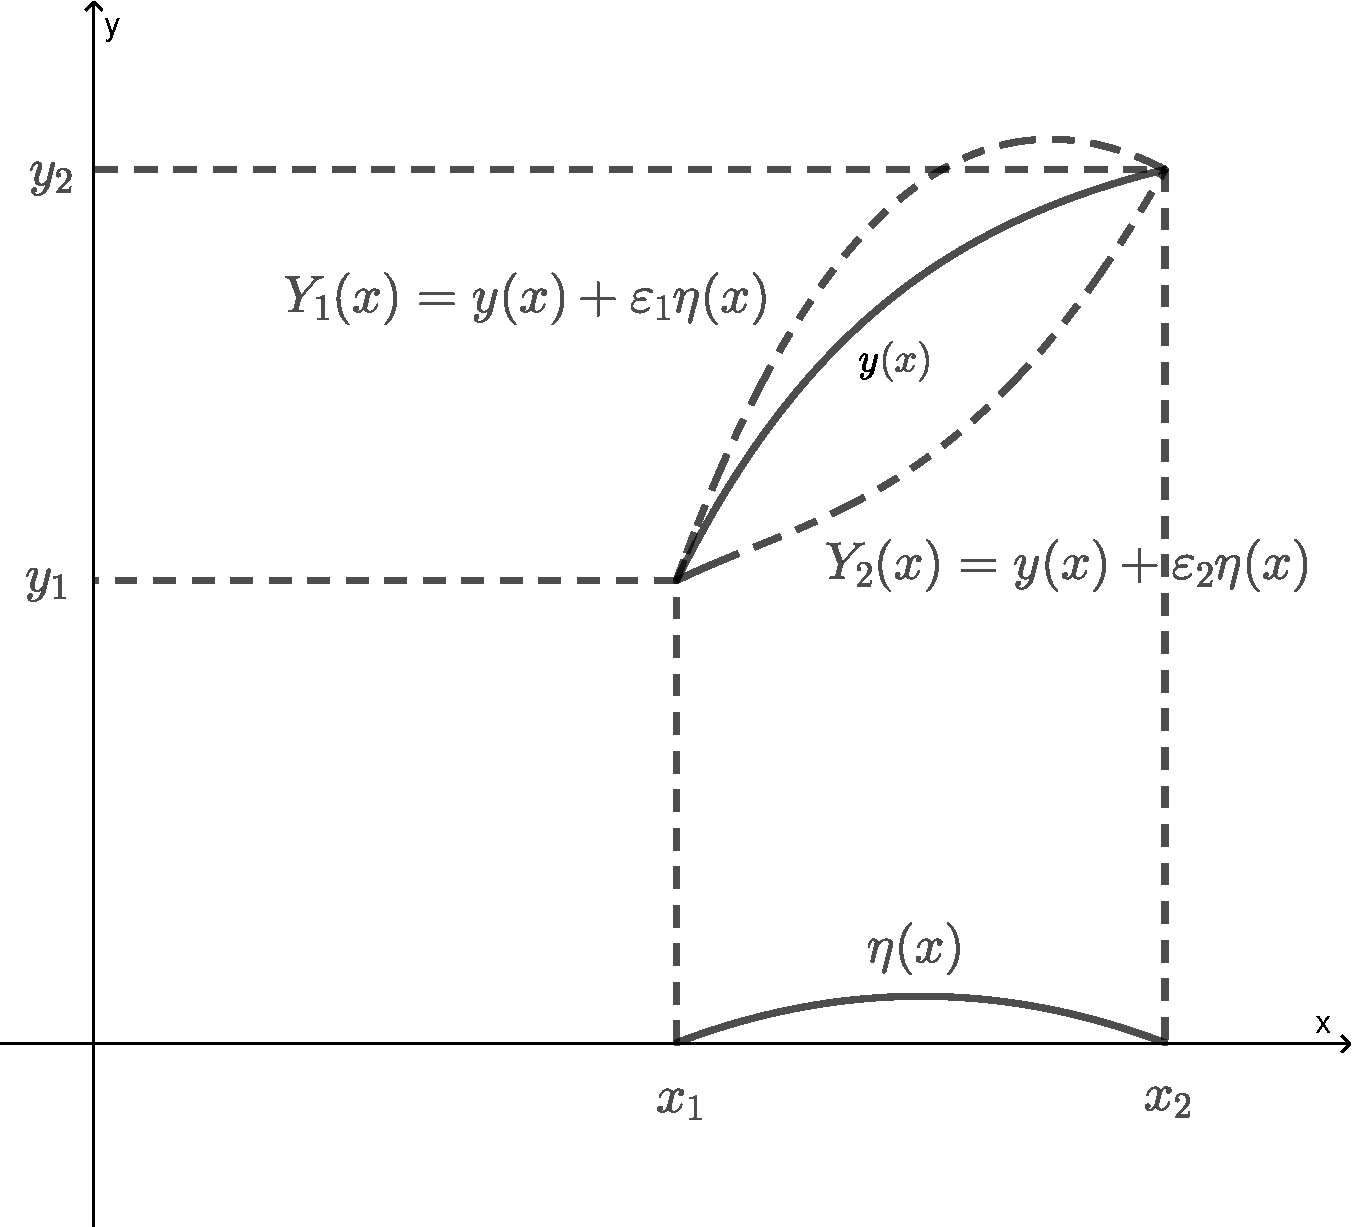
\includegraphics[width=0.5\textwidth, angle=0]{../figuras/cap_calcvar/figura_001.pdf}
	\label{fig:test_01}
	\legend{\ABNTEXfontereduzida Fonte: Elaborada pelo autor, 2019.}
\end{figure}

%\textit{\color{red}Substituir essa imagem por um desenho plotado com O Tikz/PGF.}

Reescrevendo a integral (\ref{eqn:int_funcional}) utilizando as funções aproximadoras definidas, tem-se
\begin{equation}\label{eqn:int_funcional_approx}
I(\varepsilon)=\int_{x_1}^{x_2}f(x, Y, Y')dx\text{.}
\end{equation}

Note que a função procurada $y(x)$ é o membro da família $Y(x)$ quando $\varepsilon = 0$. Ou seja, se $\varepsilon = 0$ pode-se substituir $Y$ e $Y'$ por $y$ e $y'$, respectivamente. Deste modo, a integral (\ref{eqn:int_funcional_approx}) fornece os mesmos extremos que a (\ref{eqn:int_funcional}) quando $\varepsilon=0$.

A condição necessária para que uma função de uma variável real tenha um extremo em algum ponto é que sua primeira derivada se anule nesse ponto. Então, é necessário que
\begin{equation}\label{eqn:cap_calcvar_condition}
I'(0)=0\text{.}
\end{equation}

Utilizando a Regra de Leibniz (Teorema \ref{teorema:regra_de_leibniz} do Apêndice \ref{apend:regra_de_leibniz}), a derivada de (\ref{eqn:int_funcional_approx}) pode ser escrita como
$$I'(\varepsilon)=\int_{x_1}^{x_2} \frac{\partial f}{\partial \varepsilon} (x, Y, Y') dx \text{,}$$
e, aplicando regra da cadeia, obtêm-se
$$I'(\varepsilon)=\int_{x_1}^{x_2}\left ( \frac{\partial f}{\partial x}\frac{\partial x}{\partial \varepsilon} + \frac{\partial f}{\partial Y} \frac{\partial Y}{\partial \varepsilon} + \frac{\partial f}{\partial Y'} \frac{\partial Y'}{\partial \varepsilon} \right )dx\text{,}$$
onde o primeiro termo do integrando é nulo, dado ao fato de que $x$ independe de $\varepsilon$, portanto $\dfrac{\partial x}{\partial \varepsilon}=0$, ou seja,
\begin{equation}\label{eqn:cap_calcvar_chain_rule}
I'(\varepsilon)=\int_{x_1}^{x_2}\left ( \frac{\partial f}{\partial Y}\frac{\partial Y}{\partial \varepsilon} + \frac{\partial f}{\partial Y'}\frac{\partial Y'}{\partial \varepsilon} \right ) dx \text{.}
\end{equation}

Derivando \eqref{eqn:cap_calcvar_eq_approx} em função de $\varepsilon$, tem-se $\frac{\partial Y}{\partial \varepsilon}=\frac{\partial y}{\partial \varepsilon}+\frac{\partial}{\partial \varepsilon}(\varepsilon \eta)$, de onde conclui-se que $\frac{\partial Y}{\partial \varepsilon}=\eta$, pois $y$ e $\eta$ independem de $\varepsilon$. O mesmo acontece com \eqref{eqn:cap_calcvar_eq_approx_diff}, donde verifica-se que $\frac{\partial Y'}{\partial \varepsilon}=\eta'$. Deste modo, de \eqref{eqn:cap_calcvar_chain_rule}, obtêm-se a integral
$$I'(\varepsilon)=\int_{x_1}^{x_2}\left ( 
	\frac{\partial f}{\partial Y} \eta +
	\frac{\partial f}{\partial Y'} \eta '
\right )dx \text{.}
$$

Para calcular $I'(0)$, tem-se que $\varepsilon=0$ e, então, podemos trocar $Y$ e $Y'$ por $y$ e $y'$, respectivamente, obtendo
$$
I'(0)=\int_{x_1}^{x_2}\left (
	\frac{\partial f}{\partial y} \eta +
	\frac{\partial f}{\partial y'} \eta '
\right )dx
$$
$$
I'(0)=
	\int_{x_1}^{x_2} \frac{\partial f}{\partial y}\eta dx
	+
	\int_{x_1}^{x_2} \frac{\partial f}{\partial y'}\eta' dx \text{.}
$$

Integrando o segundo membro, por partes, tomando $u=\frac{\partial f}{\partial y'}$ e $dv=\eta'dx$ de onde obtêm-se $du=\frac{d}{dx}\left ( \frac{\partial f}{\partial y'} \right )dx$ e $v=\eta$, portanto,
$$
I'(0)=
	\int_{x_1}^{x_2} \frac{\partial f}{\partial y}\eta dx
	+
	\left (
	uv \Big|_{x_1}^{x_2} - \int_{x_1}^{x_2}vdu
	\right )
$$
\begin{equation}\label{eqn:cap_calcvar_part_integration}
I'(0)=
	\int_{x_1}^{x_2} \frac{\partial f}{\partial y}\eta dx
	+
	\left (
		\frac{\partial f}{\partial y'}\eta \Biggr|_{x_1}^{x_2} - \int_{x_1}^{x_2} \frac{d}{dx}\left ( \frac{\partial f}{\partial y'} \right ) \eta dx
	\right )
\end{equation}

Sabe-se que $\frac{\partial f}{\partial y'}\eta \Big |_{x_1}^{x_2}=0$, devido ao fato de que $\eta(x_1)=\eta(x_2)=0$, portanto, \eqref{eqn:cap_calcvar_part_integration} pode ser reescrita como
$$
I'(0)=
	\int_{x_1}^{x_2} \frac{\partial f}{\partial y}\eta dx
	-
	\int_{x_1}^{x_2} \frac{d}{dx} \left ( \frac{\partial f}{\partial y'} \right ) \eta dx
$$
$$
I'(0)=\int_{x_1}^{x_2}\left (
	\frac{\partial f}{\partial y} -
	\frac{d}{dx}
	\left (
		\frac{\partial f}{\partial y'}
	\right )
\right )\eta dx
$$
que, a partir da condição necessária (\ref{eqn:cap_calcvar_condition}), deve ser igualada a $0$:
$$
I'(0)=\int_{x_1}^{x_2}\left (
	\frac{\partial f}{\partial y} -
	\frac{d}{dx}
	\left (
		\frac{\partial f}{\partial y'}
	\right )
\right )\eta dx = 0	\text{.}
$$
permitindo, pelo Lema \ref{lema:cap_calcvar_lema_1}, obter a seguinte equação:
\begin{equation}\label{eqn:cap_calcvar_euler_lagrange}
\frac{\partial f}{\partial y} - \frac{d}{dx} \left ( \frac{\partial f}{\partial y'} \right )=0 \text{.}
\end{equation}

A equação diferencial parcial \eqref{eqn:cap_calcvar_euler_lagrange} é chamada de equação de Euler-Lagrange e permite encontrar uma função $f$ que maximiza ou minimiza a integral (\ref{eqn:int_funcional}).

%\textit{\color{red}(Necessário?) Falar sobre a generalização da equação de Euler-Lagrange para $n$ variáveis.}
%\section{Generalização da Equação de Euler-Lagrange}


% ----------------------------------------------------------
% PARTE
% ----------------------------------------------------------
%\part{Preparação da pesquisa}
% ----------------------------------------------------------

% ---
% Capitulo com exemplos de comandos inseridos de arquivo externo 
% ---
%\include{abntex2-modelo-include-comandos}
% ---

% ----------------------------------------------------------
% PARTE
% ----------------------------------------------------------
%\part{Referenciais teóricos}
% ----------------------------------------------------------

\iffalse
% ---
% Capitulo de revisão de literatura
% ---
\chapter{Lorem ipsum dolor sit amet}
% ---

% ---
\section{Aliquam vestibulum fringilla lorem}
% ---

\lipsum[1]

\lipsum[2-3]

\lipsum[1]

\lipsum[2-3]

\lipsum[1]

\lipsum[2-3]

\lipsum[1]

\lipsum[2-3]

\lipsum[1]

\lipsum[2-3]

\lipsum[1]

\lipsum[2-3]

% ----------------------------------------------------------
% PARTE
% ----------------------------------------------------------
\part{Resultados}
% ----------------------------------------------------------

% ---
% primeiro capitulo de Resultados
% ---
\chapter{Lectus lobortis condimentum}
% ---

% ---
\section{Vestibulum ante ipsum primis in faucibus orci luctus et ultrices
posuere cubilia Curae}
% ---

\lipsum[21-22]

\subsection{TEstando subseção}

\subsubsection{Mais uma subseção.}

\subsubsubsection{ Chega de subsubseção.}


% ---
% segundo capitulo de Resultados
% ---
\chapter{Nam sed tellus sit amet lectus urna ullamcorper tristique interdum
elementum}
% ---

% ---
\section{Pellentesque sit amet pede ac sem eleifend consectetuer}
% ---

\lipsum[24]

% ----------------------------------------------------------
% Finaliza a parte no bookmark do PDF
% para que se inicie o bookmark na raiz
% e adiciona espaço de parte no Sumário
% ----------------------------------------------------------
\phantompart

% ---
% Conclusão
% ---
\chapter{Conclusão}
% ---

\lipsum[31-33]

\fi

% ----------------------------------------------------------
% ELEMENTOS PÓS-TEXTUAIS
% ----------------------------------------------------------
\postextual
% ----------------------------------------------------------

% ----------------------------------------------------------
% Referências bibliográficas
% ----------------------------------------------------------
\bibliography{abntex2-modelo-references}

% ----------------------------------------------------------
% Glossário
% ----------------------------------------------------------
%
% Consulte o manual da classe abntex2 para orientações sobre o glossário.
%
%\glossary

% ----------------------------------------------------------
% Apêndices
% ----------------------------------------------------------

% ---
% Inicia os apêndices
% ---
\begin{apendicesenv}

% Imprime uma página indicando o início dos apêndices
\partapendices

% Apêndice A
\chapter{Regra de Leibniz}
\label{apend:regra_de_leibniz}
{
	Para encontrar a equação de Euler-Lagrande faz-se necessário derivar uma integral. A ferramenta matemática que permite tal feito é chamada de Regra de Leibniz (Ou Derivação sob o sinal de integral) e será enunciada e demonstrada neste Apêndice. O texto deste apêndice foi elaborado com base em \citeonline{analise_elon2}.

	\begin{definicao}
		Um conjunto $K\subset \mathbb{R}^n$ é compacto se, e somente se, toda sequência de pontos em $K$ possui uma subsequência que converge para um ponto de $K$.
	\end{definicao}

	\begin{teorema}
		\label{teorema:func_uniformemente}
		Seja $f:X\times K \longrightarrow \mathbb{R}^n$ contínua, onde $K$ é compacto. Fixemos $x_0 \in X$. Para todo $\varepsilon > 0$, existe um $\delta > 0$ tal que $x\in X$, $|x-x_0|<\delta \Longrightarrow |f(x, \alpha)-f(x_0,\alpha)|<\varepsilon$, seja qual for $\alpha \in K$.
		\begin{proof}
		Suponha que o teorema não seja válido, então existiriam $\varepsilon > 0$ e sequências de pontos $x_k\in X$, $\alpha_k \in K$ tais que $|x_k-x_0|<\frac{1}{k}$ e $|f(x_k,\alpha_k)-f(x_0,\alpha_k)|\geqslant \varepsilon$. Passando a uma subsequência, se necessário e admitindo que $\lim \alpha_k=\alpha \in K$, devido ao fato de que o conjunto $K$ é compacto.
		
		Como, $|x_k-x_0|<\frac{1}{k}$, $-\frac{1}{k}<x_k-x_0<\frac{1}{k}$, então, $x_0-\frac{1}{k}<x_k<x_0+\frac{1}{k}$, e, como $\lim \left (x_0-\frac{1}{k} \right ) = x_0$ e $\lim \left ( x_0 + \frac{1}{k} \right )=x_0$, então, $\lim x_k=x_0$. Devido a continuidade de $f$ tem-se $\varepsilon \leqslant \lim |f(x_k,\alpha_k)-f(x_0,\alpha _k)|=|f(x_0,\alpha)-f(x_0,\alpha)|=0$, uma contradição, pois da hipótese $\varepsilon >0$.
		\end{proof}
	\end{teorema}
	
	\begin{teorema}[Derivação sob o sinal de integral ou Regra de Leibniz]
		\label{teorema:regra_de_leibniz}
		Dado $U\subset \mathbb{R}^n$, aberto, seja $f:U\times[a,b]\longrightarrow \mathbb{R}$ uma função com as seguintes propriedades:
		\begin{enumerate}
			\item Para todo $x \in U$, a função $x \longmapsto f(x,t)$ é integrável em $a \leqslant t \leqslant b$.
			\item A $i$-ésima derivada parcial $\frac{\partial f}{\partial x_i}(x,t)$ existe para cada $(x,t)\in U\times [a,b]$ e a função $\frac{\partial f}{\partial x_i}:U\times [a,b]\longrightarrow \mathbb{R}$ assim definida é contínua.
		\end{enumerate}
		Então a função $\varphi: U\longrightarrow \mathbb{R}$ dada por
		$$\varphi(x)=\int_a^b f(x,t)dt\text{,}$$
		possui $i$-ésima derivada parcial em cada ponto $x\in U$, sendo
		$$\frac{\partial \varphi}{\partial x_i}(x)=\int_a^b \frac{\partial f}{\partial x_i}(x,t)dt\text{.}$$

		\begin{proof}
			Considere
			$$
			\frac{\varphi(x+se_i)-\varphi(x)}{s}
			=
			\int_a^b \frac{f(x+se_i, t)-f(x,t)}{s} dt\text{,}
			$$
			de onde subtraindo $\int_a^b \frac{\partial f}{\partial x_i}(x,t) dt$ de ambos os lados, tem-se
			\begin{equation}
			\label{eqn:anexo_leibniz_r1}
			\frac{\varphi(x+se_i)-\varphi(x)}{s}
			- \int_a^b \frac{\partial f}{\partial x_i}(x,t) dt
			=
			\int_a^b \left [ 
				\frac{f(x+se_i, t)-f(x,t)}{s} 
				- \frac{\partial f}{\partial x_i}(x,t)
			\right ] dt
			\end{equation}
			
			Pelo Teorema do Valor Médio para funções reais, existe $\theta \in [0,1]$ de modo que
			$$
				\frac{f(x+se_i,t)-f(x,t)}{s}=\frac{\partial f}{\partial x_i}(x+\theta s e_i,t)\text{,}
			$$
			onde $\theta \in [0,1]$ garante que $\theta s$ esteja entre $]0, s[$, satisfazendo as condições do Teorema do Valor Médio. Assim, de \eqref{eqn:anexo_leibniz_r1} tem-se
			%donde pode-se escrever \eqref{eqn:anexo_leibniz_r1} como
			\begin{equation}
				\label{eqn:anexo_leibniz_voltas}
				\frac{\varphi(x+se_i)-\varphi(x)}{s}
				- \int_a^b \frac{\partial f}{\partial x_i}(x,t) dt
				=
				\int_a^b \left [
					\frac{\partial f}{\partial x_i}(x+\theta s e_i, t)-\frac{\partial f}{\partial x_i}(x,t)
				\right ] dt\text{.}
			\end{equation}
			
			Como $\frac{\partial f}{\partial x_i}$ é contínua e $[a,b]$ é compacto, pelo Teorema \ref{teorema:func_uniformemente}, para todo $\varepsilon > 0$, existe um $\delta > 0$, de modo que
			\begin{equation}
				\label{eqn:anexo_leibniz_ineq_func_unif}
				|s|<\delta \Longrightarrow
				\left | 
					\frac{\partial f}{\partial x_i} (x+\theta s e_i, t) - \frac{\partial f}{\partial x_i}(x,t)
				\right | < \frac{\varepsilon}{b-a}
			\end{equation}
			seja qual for $t \in [a,b]$.
			
			Usando o fato de que $|\int_a^b f(x)dx| \leqslant \int_a^b |f(x)| dx$, obtêm-se
			$$
			\left |
				\int_a^b \left [
					\frac{\partial f}{\partial x_i}(x+\theta s e_i, t)-\frac{\partial f}{\partial x_i}(x,t)
				\right ] dt
			\right |
			\leqslant
			\int_a^b\left |
				\frac{\partial f}{\partial x_i}(x+\theta s e_i, t)-\frac{\partial f}{\partial x_i}(x,t)
			\right | dt\text{,}
			$$
			e, utilizando \eqref{eqn:anexo_leibniz_ineq_func_unif}, tem-se a inequação
			$$
			\left |
				\int_a^b \left [
					\frac{\partial f}{\partial x_i}(x+\theta s e_i, t)-\frac{\partial f}{\partial x_i}(x,t)
				\right ] dt
			\right |
			<
			\int_a^b \frac{\varepsilon}{b-a} dt
			$$
			\begin{equation}
				\label{eqn:anexo_leibniz_ineq_limit}
				\left |
					\int_a^b \left [
						\frac{\partial f}{\partial x_i}(x+\theta s e_i, t)-\frac{\partial f}{\partial x_i}(x,t)
					\right ] dt
				\right |
				< \varepsilon \text{.}
			\end{equation}
			
			De \eqref{eqn:anexo_leibniz_voltas} e \eqref{eqn:anexo_leibniz_ineq_limit}, verifica-se que
			$$
				|s|<\delta \Longrightarrow
				\left |
					\frac{\varphi(x+se_i)-\varphi(x)}{s}
					- \int_a^b \frac{\partial f}{\partial x_i}(x,t) dt
				\right |
				< \varepsilon\text{,}
			$$
			que é, a definição formal do limite
			$$
				 \lim_{s\to 0} \frac{\varphi (x+se_i)-\varphi(x)}{s}= \int_a^b \frac{\partial f}{\partial x_i} (x, t)dt \text{,}
			$$
			ou seja,
			$$
				\frac{\partial \varphi}{\partial x_i}(x)=\int _a^b \frac{\partial f}{\partial x_i}(x,t)dt\text{.}
			$$
		\end{proof}
	\end{teorema}
	
	\iffalse
	\begin{teorema}
		\label{teorema:regra_de_leibniz}
		Considere uma função $f:[a,b]\times [c,d] \longrightarrow \mathbb{R}$ e suponha que a derivada parcial $\frac{\partial f}{\partial p}(x,p)$ existe e é contínua em $[a,b]\times [c,d]$. Se a integral
		$$F(p)=\int_a^b f(x, p)dx$$
		existe para todo $p\in [c,d]$, então $F(p)$ é diferenciável e
		$$F'(p)=\int_a^b \frac{\partial f}{\partial p} (x, p)dx \text{.}$$
		\textit{\color{red} Estudar, entender e demonstrar a regra de Leibiniz.}
	\end{teorema}
	\fi
}

\end{apendicesenv}
% ---


\iffalse
% ----------------------------------------------------------
% Anexos
% ----------------------------------------------------------

% ---
% Inicia os anexos
% ---
\begin{anexosenv}

% Imprime uma página indicando o início dos anexos
\partanexos

% ---
\chapter{Morbi ultrices rutrum lorem.}
% ---
\lipsum[30]

% ---
\chapter{Cras non urna sed feugiat cum sociis natoque penatibus et magnis dis
parturient montes nascetur ridiculus mus}
% ---

\lipsum[31]

% ---
\chapter{Fusce facilisis lacinia dui}
% ---

\lipsum[32]

\end{anexosenv}

\fi

%---------------------------------------------------------------------
% INDICE REMISSIVO
%---------------------------------------------------------------------
\phantompart
\printindex
%---------------------------------------------------------------------

\end{document}
